\chapter{Ethernet}
\label{chap:ethernet}

\paragraph{\acs{MAC} addresses}
   \index{MAC address@\acs{MAC} address}
A \ac{MAC} address is a unique identifier that is assigned to a \ac{NIC} for use as an address in communication within a network segment.
   \iacs{NIC}
\ac{MAC} addresses are primarily assigned by device manufacturers and stored in read-only memory.
As such they are often referred to as the \emph{burned-in address}, the \emph{hardware address}, or the \emph{physical address}.
Nowadays it is often possible to change the \acs{MAC} adddress used on an interface.

\paragraph{48 bits}
A \ac{MAC} address consists of 48~bits, most often displayed as six groups of two hexadecimal digits, separated by hyphens or colons (e.g.~02:\-00:\-33:\-aa:\-bb:\-cc).
Sometimes the address is displayed as three groups of four hexadecimal digits, separated by dots, e.g. 0200.33aa.bbcc.%
   \footnote{Hexadecimal numbers are not case-sensitive, the value of `4F' is equivalent to that of `4f.'}

\paragraph{\acf{OUI}}
   \iacs{OUI}
The first twenty-four bits of a \ac{MAC} address identify the vendor or manufacturer of the network card.
\Acp{OUI} are purchased from the \acs{IEEE} registration authority by the vendor.
   \iacs{IEEE}
They are used to make sure that -- in theory at least -- every \acs{MAC} address is unique.

\extrat{This is not the complete truth} about \acs{MAC} addresses as there are two special bits in the \acs{OUI}.
The last two bits of the first byte have a special meaning.
The right-most bit indicates a multicast (or broadcast) address when set to one.
The left-most of those two special bits indicates a locally administered \acs{MAC} address when set to one.
The term `locally administered' means that the administrator of the machine has manually set the \acs{MAC} address -- and it is thus not guaranteed to be globally unique.
In this case, the first three bytes are not an \acl{OUI}.
See \cref{fig:mac-format} for the complete picture of a \acs{MAC} address.


\begin{figure}
\centering
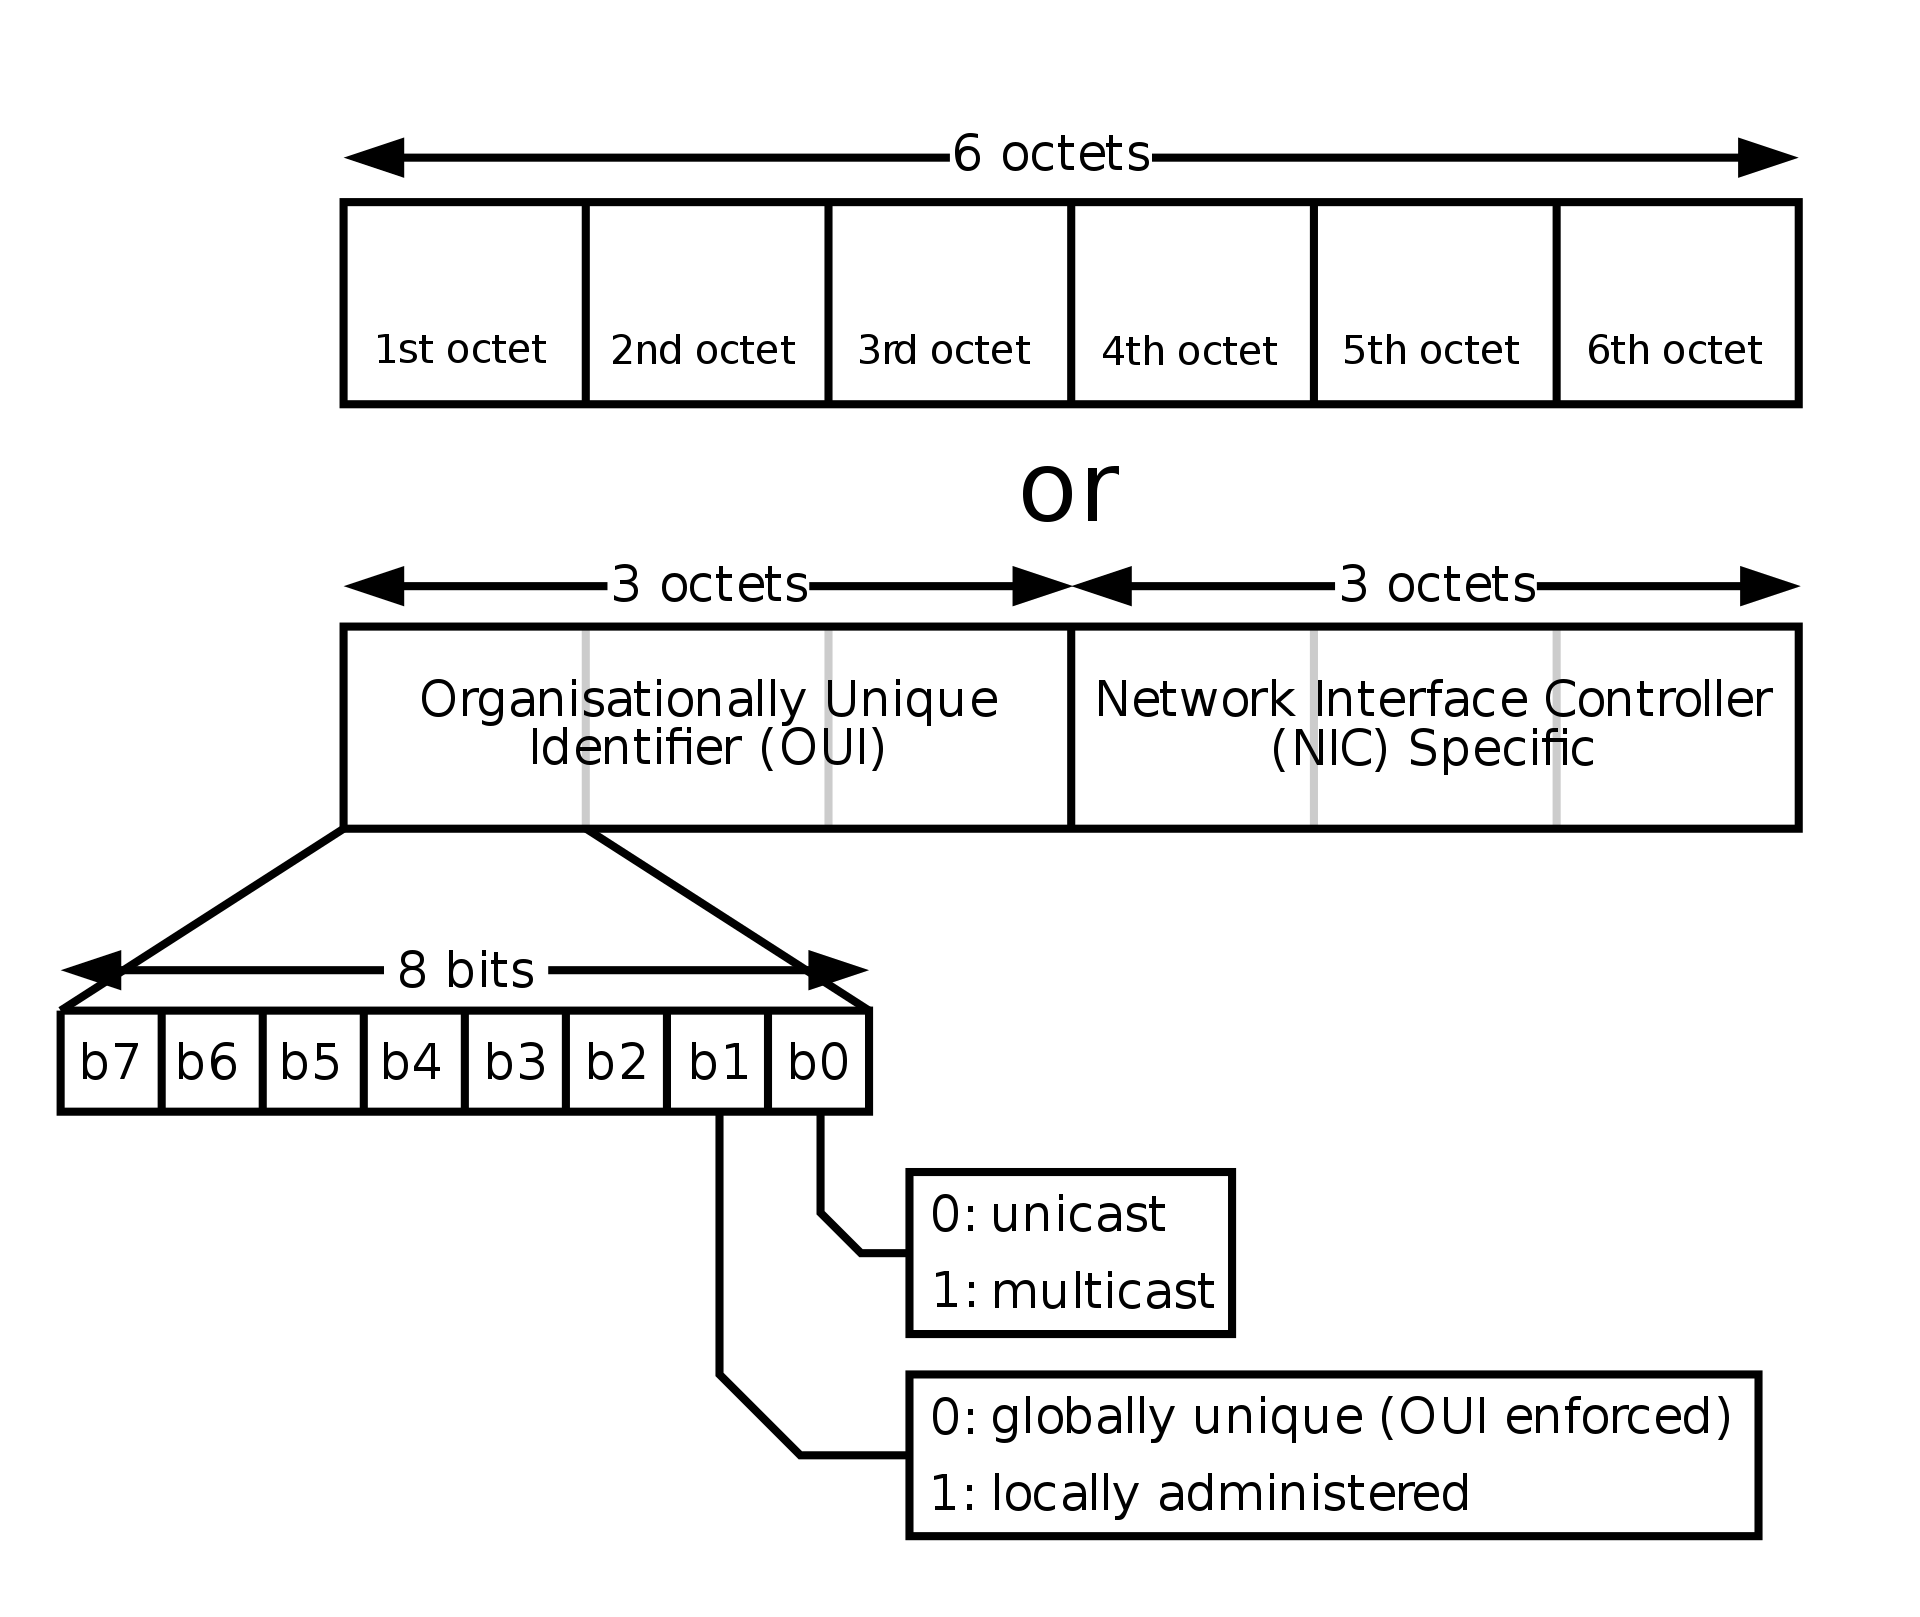
\includegraphics[width=\textwidth]{images/ethernet/mac-address-format.png}
\caption[The format of a \acs{MAC} address]{The \acs{MAC} address consists of two parts with the first part having two bits with special meaning}
\label{fig:mac-format}
\end{figure}

\paragraph{1522 bytes}
   \index{frame!size}
   \iacs{MTU}
Ethernet frames have a maximum size of 1522~bytes and a minimum frame size of 64~bytes.
Twenty-two bytes are used by the Ethernet header (18~bytes) and trailer (4~bytes) so that the encapsulated \acs{IP} packet has a maximum size of 1500~bytes.
This is also called the \acf{MTU}.


\paragraph{Ethernet header}
   \index{Ethernet!header}
The standard length of the Ethernet header is 14~bytes, however, when using \acs{VLAN} tagging, it is extended to 18~bytes.
It contains the source and destination \acs{MAC} addresses, a field designated for either the \emph{ethertype} or the length of the data payload,%
   \footnote{%
      The Ethernet version 2 or \acs{DIX} frame, is the most common type in use today.
      It uses the two-byte field to store an ethertype value.
      The \acs{IEEE} 802.3 Ethernet frame stores the length of the data payload into this field and an 802.2 \SC{LLC} header follows the 802.3 header.

      When the length is given, the driver must determine the protocol by looking into the frame's content.
      When the protocol is given, the length must be calculated by counting the bytes received on the wire.
   }
and an optional \SC{802.1Q} tag containg \acs{VLAN} and \acs{CoS} information.

The ethertype field is a two-byte field in the Ethernet header that is used to identify the type of data that is being transmitted in the Ethernet frame.
   \index{ethertype}
It is used to indicate the protocol that is encapsulated in the payload of the Ethernet frame.
The ethertype field is located immediately after the destination and source \acs{MAC} addresses in the Ethernet header.



%\paragraph{802.1Q tag}
% TODO: Expand on the ethertype and the 802.1Q tag.

%\begin{figure}
%   \centering
%   TODO: Ethernet frame
%   \caption{An Ethernet frame}
%   \label{fig:ethernet-frame}
%\end{figure}

\paragraph{Ethernet trailer}
   \index{Ethernet!trailer}
   \iacs{FCS}
   \iacs{CRC}
The frame ends with a \acf{FCS}, which is a 32-bit \acf{CRC} used to detect any in-transit corruption of data.

\extrap{\acl{CRC}}
A \acs{CRC} is an error-detecting code commonly used in digital networks and storage devices to detect accidental changes to digital data.
Blocks of data entering these systems get a short check value attached, based on the remainder of a polynomial division of their contents.
On retrieval, the calculation is repeated and, in the event the check values do not match, corrective action can be taken against data corruption.
A \acs{CRC} can be used for error correction.

\paragraph{jumbo frames} 
   \index{frame!jumbo}
   \index{frame!size}
   \iacs{MTU}
Some implementations of Gigabit Ethernet and other higher-speed variants of Ethernet support larger frames, known as jumbo frames.%
   \footnote{%
      Any Ethernet frame that is larger that {1500}~bytes is called a jumbo frame.
      Those frames that are only just larger are called \emph{baby giants}.
      Two examples would be \acs{VLAN} tagging and \SC{Q}-in-\SC{Q} tagging which have an \acs{MTU} of {1504} and {1508}~bytes respectively.}
These frames can be up to 9000 bytes in size.%
   \footnote{For example the Juniper QFX series of switches support frames up to {9216}~bytes.}
Jumbo frames are mainly used in data centres as the use of these larger frames require all intermediate devices to support them which is impossible to require from devices on the internet.
   \index{data centre}


\section{Ethernet switch}
\label{sec:ethernet-switch}

\paragraph{hub}
   \index{hub}
   \index{half duplex}
An Ethernet hub has multiple \ac{IO} ports, in which a signal introduced at the input of any port appears at the output of every other port.
A hub works at the physical layer (layer~1) of the \ac{OSI} model.
Because hubs are nothing more than physical interconnections between the cables, when two or more hosts transmit at the same time, their messages become garbled: a collision occurs.
This means that all devices interconnected to each other through the hub form a single collision domain.
The network forms a half-duplex system: only one device can transmit at any moment in time.

\paragraph{collision domain}
   \index{collision domain}
A collision domain is a network segment connected by a shared medium or through repeaters where simultaneous data transmissions collide with one another.
The collision domain applies particularly in wireless networks, but also affected early versions of Ethernet.
A network collision occurs when more than one device attempts to send a packet on a network segment at the same time.
Members of a collision domain may be involved in collisions with one another.
Devices outside the collision domain do not have collisions with those inside.

\paragraph{bridge}
   \index{bridge}
A bridge uses a table called a \acf{FIB} to control the forwarding of frames between network segments.
The table starts empty and entries are added as the bridge receives frames.
If a destination address is not found in the table, the frame is flooded to all other ports of the bridge, flooding the frame to all segments except the one from which it was received.
In the context of a two-port bridge, the \acl{FIB} can be seen as a filtering database.

\paragraph{switch}
   \index{switch}
A basic switch is a multi-port bridge.
More advanced switches have many additional features, see managed switches on p.~\pageref{par:ethernet-switch-managed}.

\paragraph{buffers}
   \index{buffer}
Assume a switch receives two Ethernet frames at the same time, one on its first interface, the second on its second interface.
Both have to be sent out through its third interface.
It is not possible to send both out at the same time as the signals would interfere with each other.
Thus one of the frames needs to be stored in a temporary buffer while the other is being sent over the wire.


\extrap{store-and-forward}
   \index{forwarding!store-and-forward}
   \index{forwarding!cut-through}
When a switch the receives the entire Ethernet frame into its buffer, calculates and verifies the \acs{FCS}, and only then forwards the frame further towards its destination, it is called \emph{store-and-forward} switching.
In contrast, with \emph{cut-through} switching the switch starts sending out the Ethernet frame as soon as the destination \acs{MAC} address (and optionally its \acs{VLAN}) are read it.
This way the switch introduces less latency into the network transmission but it is possible corrupt Ethernet frames -- whose \acs{FCS} is no longer correct -- are being forwarded.

\paragraph{\acs{MAC}-address table}
   \index{MAC-address table@\acs{MAC}-address table}
   \index{switch}
A network switch learns the identities of connected devices from incoming frames and then only forwards data to the port connected to the device to which it is addressed.
These learnt \acs{MAC} addresses are stored in the \ac{MAC}-address table or \acf{FIB}.

The \acs{MAC}-address table contains the interface number that the frame came in on, the learnt \acs{MAC} address, the \acs{VLAN} that the frame belongs to, and a timer.
The timer serves to age out entries that are not used for a specific period of time.
By default, this timeout is three hundred seconds on a Cisco switch.

\paragraph{time to live?}
   \index{network loop}
   \iacs{TTL}
Ethernet has no \acl{TTL} field so when a loop gets created in the network, the frames will keep traversing the network, bringing the entire network down.

\paragraph{\acf{STP}}
   \iacs{STP}
   \index{loops!loop-free topology}
   \index{backup link (\acs{STP})}
   \index{broadcast!radiation}
The \acl{STP} is a network protocol that builds a loop-free logical topology for Ethernet networks.
The basic function of \acs{STP} is to prevent bridge loops and the broadcast radiation that results from them.
\acs{STP} also allows a network design to include backup links providing fault tolerance if an active link fails.

\paragraph{flavours of \acs{STP}}
   \index{STP@\acs{STP}!flavours}
   \iacs{RSTP}
   \iacs{PVST}
In 2001, the \acs{IEEE} introduced \acf{RSTP} as 802.1w.
\acs{RSTP} provides significantly faster recovery in response to network changes or failures, introducing new convergence behaviors and bridge port roles to do this.
\acs{RSTP} was designed to be backwards-compatible with standard \acs{STP}.

\acs{STP} and \acs{RSTP} do not segregate switch ports by \acs{VLAN}.
However, in Ethernet switched environments where multiple \acsp{VLAN} exist, it is often desirable to create multiple spanning trees so that traffic on different \acsp{VLAN} uses different links.
Before the \acs{IEEE} published an \acs{STP} standard for \acsp{VLAN}, a number of vendors who sold \acs{VLAN}-capable switches developed their own \acs{STP} versions that were \acs{VLAN} capable.
Cisco developed, implemented and published the proprietary \acf{PVST} protocol and \acs{PVST+} which uses \SC{802.1Q} \acs{VLAN} encapsulation.
   \iacs{PVST}
   \iacs{PVST+}
Both standards implement a separate spanning tree for every \acs{VLAN}.

Juniper Networks in turn developed and implemented its \acf{VSTP} to provide compatibility with Cisco's \acs{PVST}, so that the switches from both vendors can be included in one network.
Cisco also published a proprietary version of \acf{RSTP}.
   \iacs{VSTP}
It creates a spanning tree for each \acs{VLAN}, just like \acs{PVST}.
Cisco refers to this as \acf{RPVST}.
   \iacs{RPVST}


\paragraph{\acf{MSTP}}
The downside of all these per-\acs{VLAN} protocols is that you can have up to 4094~\acsp{VLAN} and thus these protocols will build up to 4094~topologies.
It is however highly unlikely that there will be enough redundancy in the network to accomodate more than two distinct topologies.
\acs{MSTP} solves this problem by grouping multiple \acsp{VLAN} and creating distinct topologies for each group.
This greatly cuts down on the resources the switch needs to allocate for these topologies.


\section{Advanced features}
\label{sec:ethernet-advanced-features}

\paragraph{\acf{LAG}}
   \iacs{LAG}
Link aggregation is the combining (aggregating) of multiple network connections in parallel by any of several methods, in order to increase throughput beyond what a single connection could sustain, to provide redundancy in case one of the links should fail, or both.
A \ac{LAG} is the combined collection of physical ports.
Other umbrella terms used to describe the concept include trunking%
   \footnote{Not to be confused with \acs{VLAN} trunking which is something entirely different than link aggregation trunking.}%
, bundling, bonding, channeling, ether-channel or teaming.


\paragraph{switch stack}
A stackable switch is a network switch that is fully functional operating standalone but which can also be set up to operate together with one or more other network switches, with this group of switches showing the characteristics of a single switch but having the port capacity of the sum of the combined switches.
The term \emph{stack} refers to the group of switches that have been set up in this way.
The common characteristic of a stack acting as a single switch is that there is a single \acs{IP} address for remote administration of the stack as a whole, not an \acs{IP} address for the administration of each unit in the stack.

\paragraph{managed switch}
\label{par:ethernet-switch-managed}
   \index{switch!managed}
   \iacs{CLI}
   \index{serial console}
   \iacs{SNMP}
   \index{port mirroring}
Managed switches have one or more methods to modify the operation of the switch.
Common management methods include: a \ac{CLI} accessed via serial console, Telnet or \ac{SSH} (see \vref{chap:applications}), an embedded \ac{SNMP} agent allowing management from a remote console or management station, or a web interface for management from a web browser.
Examples of configuration changes that one can do from a managed switch include: enabling features such as \ac{STP} or port mirroring, setting port bandwidth, creating or modifying \acp{VLAN}, etc.

We will take a quick look at the following features of managed switches:
\begin{inlinelist}
\item \aclp{VLAN},
\item port security and \SC{802.1X},
\item \acs{DHCP} snooping, and
\item \acl{DAI}.
\end{inlinelist}

\paragraph{\acs{VLAN}}
      \iacs{VLAN}
      \index{broadcast domain}
A \acf{VLAN} is any broadcast domain that is partitioned and isolated in a computer network at the data link layer.
\acp{VLAN} work by applying tags to network frames and handling these tags in networking systems -- creating the appearance and functionality of network traffic that is physically on a single network but acts as if it is split between separate networks.
In this way, \acp{VLAN} can keep network applications separate despite being connected to the same physical network, and without requiring multiple sets of cabling and networking devices to be deployed.


\paragraph{access port}
   \index{access port}
An access port is an interface that is assigned to only one \acs{VLAN}.
Network frames sent and received on this port are not tagged with a \acs{VLAN} \SC{ID}.
This type of interface is used towards end hosts such as printers, laptops, and workstations as they often do not understand \SC{802.1Q} tags.


\paragraph{trunk port}
   \index{trunk port}
A trunk port is an interface that is assigned to more than one \acs{VLAN}.
For the switch to be able to assign the network frame to the correct virtual network, all frames must be tagged with the correct \acs{VLAN} number.

\extrap{\SC{802.1Q}}
   \index{frame!size}
   \iacs{MTU}
\SC{802.1Q} adds a 32-bit field between the source \acs{MAC} address and the ethertype field of the original frame.
Under \SC{802.1Q}, the maximum frame size is extended from 1518~bytes to 1522~bytes.
The minimum frame size remains 64~bytes.
Two bytes are used for the \acf{TPID}, the other two bytes for \acf{TCI}.
The \acs{TCI} field is further divided into \acs{PCP}, \acs{DEI}, and \acs{VID}.

% TODO: include an image of the VLAN tag

The \acl{TPID} is basically just the ethertype field.
It is a 16-bit field containing the hexadecimal value of 8100 which indicates an \acs{IEEE} \SC{802.3Q}-tagged frame.
Receiving devices know that the next two bytes will contain \acs{VLAN} information and the two after that will contain the real ethertype value.

The \acs{PCP} and \acs{DEI} bits are used for quality of service and congestion control.
The \acl{VID} is a 12-bit field specifying the \acs{VLAN} to which the frame belongs.
The values of 0 and 4095 (f{}f{}f in hexadecimal) are reserved.
All other values may be used as \acs{VLAN} identifiers, allowing up to 4094~\acp{VLAN}.

\extrap{native \acs{VLAN}}
   \index{VLAN@\acs{VLAN}!native}
Should a trunk port receive frames that lack an \SC{802.3Q} tag, it is considered to belong to the \emph{native} \acs{VLAN} of that trunk port.
The network administrator can configure which \acs{VLAN} should be considered to be the native \acs{VLAN} for each interface.


\paragraph{layer-3 switch}
   \index{switch!layer-3}
   \index{switch!multi-layer switch}
As engineers continue to advance in their field, they have developed the ability to create larger and more complex chips.
This advancement allows for the integration of more complex logic into network switches.
Layer-3 switches in particular have the capability to route packets in hardware based on \acs{IP} addresses, effectively functioning as routers.
As a result, it has become increasingly convenient to implement a layer-3 switch into network infrastructure, as it combines the functionality of both routers and traditional switches.




\section{Security}

\paragraph{\acs{MAC} filtering}
   \index{MAC filtering@\acs{MAC} filtering}
   \iacs{NIC}
\ac{MAC} \emph{filtering} is a security access control method whereby the \acs{MAC} address assigned to each network card is used to determine access to the network.
\ac{MAC} filtering on a network permits and denies network access to specific devices through the use of blacklists and whitelists.
Many devices that support \acs{MAC} filtering do so on a per-device basis.
Whitelisted \ac{MAC} addresses are allowed through any port on the device and blacklisted \acs{MAC} addresses are blocked on all ports.
Other devices, such as Cisco Catalyst switches, support \acs{MAC} filtering on a port-by-port basis.
Cisco refers to \acs{MAC} filtering as port security.

\paragraph{\SC{802.1X}}
   \iacs{NAC}
\acs{IEEE} \SC{802.1X} is an \acs{IEEE} standard for \ac{PNAC}.
It provides an authentication mechanism to devices wishing to attach to a \ac{LAN} or \ac{WAN}.

\SC{802.1X} authentication involves three parties: a supplicant, an authenticator, and an authentication server.
   \index{supplicant (\acs{NAC})}
   \index{authenticator (\acs{NAC})}
   \index{authentication server (\acs{NAC})}
The supplicant is a client device (such as a laptop) that wishes to attach to the \ac{LAN} or \ac{WAN}.
The authenticator is a network device that provides a data link between the client and the network and can allow or block network traffic between the two, such as an Ethernet switch or wireless access point.
The authentication server is typically a trusted server that can receive and respond to requests for network access, and can tell the authenticator whether the connection is to be allowed, and various settings that should apply to that client's connection.
Authentication servers typically run software supporting the \ac{RADIUS} protocol and \ac{EAP} framework.
   \index{switch}
   \index{access point}
   \iacs{RADIUS}
   \iacs{EAP}

\paragraph{\acs{DHCP} snooping}
   \index{DHCP@\acs{DHCP}!snooping}
\ac{DHCP} snooping is a series of techniques applied to improve the security of a \ac{DHCP} infrastructure.
\ac{DHCP} snooping can be configured on \ac{LAN} switches to exclude rogue \ac{DHCP} servers and remove malicious or malformed \ac{DHCP} traffic.
In addition, information on hosts which have successfully completed a \ac{DHCP} transaction is accrued in a database of bindings which may then be used by other security or accounting features, such as \acl{DAI}.
   \index{DHCP@\acs{DHCP}!rogue server}

The \ac{DHCP} snooping feature performs the following activities:
\begin{itemize}
\item it validates \acs{DHCP} messages received from untrusted sources and filters out invalid messages.
\item it rate-limits \acs{DHCP} traffic both from trusted and untrusted sources.
\item it builds and maintains the \acs{DHCP} snooping database, which contains information about untrusted hosts with leased \acs{IP} addresses.
\item it utilises the \acs{DHCP} snooping binding database to validate subsequent requests from untrusted hosts.
\end{itemize}

\paragraph{\acl{DAI}}
   \index{dynamic ARP@dynamic \acs{ARP} inspection}
\Acf{DAI} is a security feature that validates \acs{ARP} packets in a network.
   \iacs{ARP}
\Acl{DAI} allows a network administrator to intercept, log, and discard \ac{ARP} packets with invalid \acs{MAC}-address-to-\acs{IP}-address bindings.
This capability protects the network from certain man-in-the-middle attacks.


\section{Review questions}

\section{Guided exercises}

\section{Practice questions}

\section{Further reading}
\textcite{lammle-ccna} is my go-to book for \acs{CCNA}-level topics such as the \acf{STP} and its variants or \acfp{LAG}.
For more -- and I do mean \emph{a lot} more -- details on \SC{802.1X} and \acf{NAC}, I would go to \textcite{woland}.
Its coauthor (McNamara) even has the nickname the \acs{ISE} queen with \acs{ISE} standing for Cisco's \acl{ISE}, an identity-based \acs{NAC} and policy-enforcement system.
